\documentclass[a4paper,12pt]{article}

\usepackage[margin=1in]{geometry}
\usepackage{tikz}
\usepackage{amssymb}
\usepackage{xcolor}
\usepackage{circuitikz}
\usepackage{graphicx}

\newcommand{\ra}{$\rightarrow$}
\newenvironment{6mini}{
  \begin{minipage}{6cm}
}{
  \end{minipage}
}

\title{\texttt{Latches and Flip Flops}\\\hrulefill}
\author{module 10}
\date{\small{10/30/2023}}

\begin{document}
    \maketitle

    \section{Memory in Digital Logic}
    These are advanced logic devices \ra~adding more memory to digital design allows for more advanced circuits. Memory is achievd in digital logic through \texttt{feedback}.
    \begin{itemize}
        \item Given a logic device, connecting its output back to its input
        \item output of a latch or flip flop is referred to as a \texttt{state}
        \item states are used to determine the output of a logic circuit that is comprised of memor elements.    
    \end{itemize}
    
        \subsection{Feedback concept}
            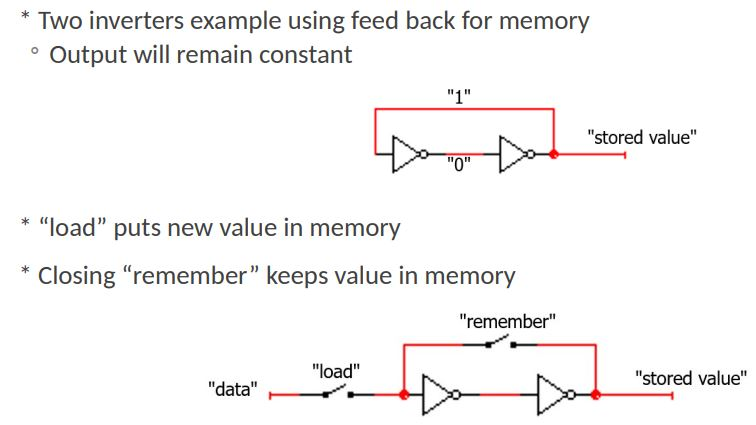
\includegraphics[width=10cm]{FeedbackConcept.JPG}
        \subsection{States}
            States define the output of logic circuits. Outputs may also depend on previous states in memory.
            \begin{itemize}
                \item Memory elements are used to remember what state a logic circuit is in
            \end{itemize}
            
    \subsection{SR Latch}
        The most basic memeory element \ra~level triggered (input is either one or zero). Latch state os either set or reset
        \begin{itemize}
            \item Latch is set: output is \textbf{1}
            \item Latch is reset: output is \textbf{0}
            \item Output(state) is denoted \(Q~\textnormal{and}~\bar{Q}\)
        \end{itemize}
        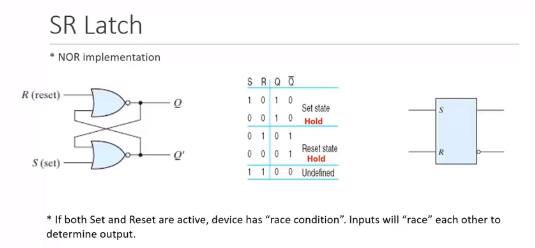
\includegraphics[width=15cm]{SRlatchDiagram1.png} \\
        It would be put into the set state with the input combination S = 1 \& R = 0, because anything NOR 1 is 0 ($\bar{Q}$).This gives 0 NOR, which is 1 ($Q$). Once the S is set 0, the state is "held", for 0 NOR 1 is 0($\bar{Q}$) and 0 Nor 0 is 1 ($Q$). The same logic can be applied to the input combination S = 0 \& R = 1, which configures the latch into the reset state.
        \begin{itemize}
            \item If both set and Reset are active, device has "race condition". Inupts will "race" each other to determine outputs.
        \end{itemize}
            \subsubsection{Adding an  Enable}
                A third input can act as a control signal, enabling o disabling the latch (getting into clocking).\\
                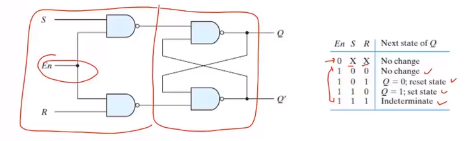
\includegraphics[width=14cm]{enabledLatch.png}. \\
                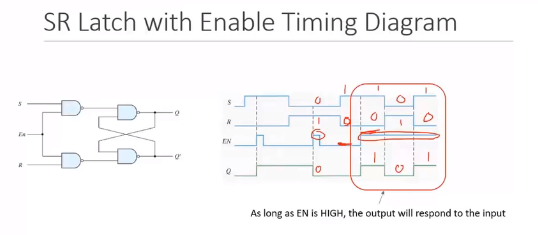
\includegraphics[width=16cm]{SRwithTiming.png}
    \subsection{Clocks}
        \begin{itemize}
            \item Series of HIGH and LOW pulses at a specific frequency
            \item cicuits can operate on the clock edges or clock level
        \end{itemize}
        \[f=\frac{1}{T}\]
            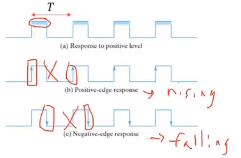
\includegraphics[width=10cm]{clocks_EdgeandLevel.png}\\
        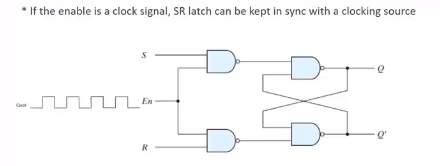
\includegraphics[width=12cm]{SRClock.png}\\
        The issue with level triggerd clock pulses is multiple transiitons can occur within a single clock pulse. \\
        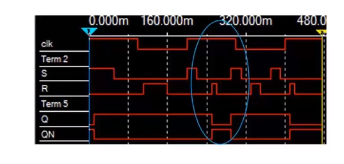
\includegraphics[width=10cm]{SRtimingDiagram.png}
    \subsection{D latch}
        connecting inputs together of SR to create D (stands for Data)
        \begin{itemize}
            \item Whenever latch is enable, Q is the value of D.
            \item Reconsiles unstable SR latch
        \end{itemize}
        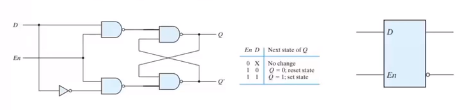
\includegraphics[width=14cm]{DlatchDiagram.png}\\
            \subsubsection{D latch timing Diagram}
                The output follows the value os D when clock is High.\\
                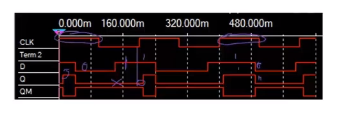
\includegraphics[width=10cm]{Dlatchtiming.png}
                 \begin{itemize}
                    \item Of course, multiple input changes can occur in one clock pulse (undesired behaviour in synchronous circuits).
                 \end{itemize}
            \subsubsection{Latch problem}
                 The output can respond to any input within an enable is active. This could cause asynchronous behaviour.\\
                 \par A solution to this is creating a transition enable (creating \texttt{flipflops})
                 \begin{itemize}
                    \item Enable is only active when transitioning from active LOW to active HIGH or vice versa
                    \item Only register input on clock's edges (rising or falling)
                \end{itemize}
                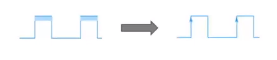
\includegraphics[width=10cm]{LeveltoEdge.png}
                
\end{document}